\documentclass[12pt,p a4paper]{class/ncku_class}

\usepackage{times}
\usepackage{CJKutf8}  %%% ZZZ %%% macro for Chinese/Japanese/Korean processing
\usepackage{CJKnumb} %%% ZZZ %%% for Chinese numbering capability

\usepackage[nospace]{cite}  % for smart citation
\usepackage{geometry}  % for easy margin settings
\usepackage{class/ncku_style} % 自定義nckuee.sty
\usepackage{booktabs}
\usepackage[pdftex]{graphicx}
\newcommand\myworkflow{pdftex}  % set the flag
\usepackage{fancyhdr}  % 借用此套件來擺放浮水印

% 啟動 fancy header/footer 套件
\pagestyle{fancy}
\fancyhead{}  % reset left, central, right header to empty
\fancyfoot[C]{\thepage} %中間 footer 擺放頁碼
\renewcommand{\headrulewidth}{0pt} % header 的直線; 0pt 則無線

% 如果不需要任何浮水印,則請把下列介於 >>> 與 <<< 之間
% 的文字行關掉 (行首加上百分號)
%% 浮水印 >>>
%
% this file is encoded in utf-8
% v2.0 (Apr. 5, 2009)
% 如果浮水印不是全篇需要,請把下列介於 >>> 與 <<<
% 的「全篇浮水印專用碼」關掉 (行首加百分號)
% 參考自 Keith Reckdahl 寫的 "Using Imported Graphics in LATEX2e" (epslatex.pdf) p.39
% 如果只有特定頁需要浮水印
% 則依該頁屬性使用下列之一的命令 
% 普通頁命令 \thispagestyle{WaterMarkPage}
% plain 頁命令 \thispagestyle{PlainWaterMarkPage}
% empty 頁命令 \thispagestyle{EmptyWaterMarkPage}


% 將重複使用的浮水印章
% 圖檔是 my_watermark.xxx
% 副檔名可以不加,可以是 latex 系統能處裡的任何格式:pdf, gif, png, jpg, eps, ...
% 某些圖檔格式在某些工作流程可能需要作前置處裡。
% 例如,pdflatex 無法直接處理 eps 檔
%  latex + dvipdfmx 無法直接處理 pdf, gif, png, jpg, 需要用 ebb 小工具程式
%  對圖檔產生 .bb 對應檔。
%
% 寬為 5.1 cm
\newsavebox{\mywatermark}
%\sbox{\mywatermark}{
\includegraphics[keepaspectratio,%
%width=5.1cm]{ncku_watermark}}

\sbox{\mywatermark}{
\includegraphics{header/ncku_watermark.jpg}}

% 將 central header 擺放浮水印的巨集指令
\newcommand{\PlaceWaterMark}{\fancyhead[C]{\setlength{\unitlength}{1in}%
\begin{picture}(0,0)%
%\put(-1,-6.2){\usebox{\mywatermark}}% 圖檔擺放的位置座標
\put(-1.35,-6.55){\usebox{\mywatermark}}% 圖檔擺放的位置座標
\end{picture}}%
}

\fancyhead{}  % reset left, central, right header to empty
%% 如果不需整篇論文都要浮水印
%% 則下面  >>> 與 <<< 之間的程式碼請關閉
%% >>> 全篇浮水印
\PlaceWaterMark  % 每一頁都有浮水印 (除了 plain、empty 頁以外)

% 重新定義 plain 頁面
% 每張 plain 頁面 (每一章的第一頁) 也加浮水印

\fancypagestyle{plain}{%
\fancyhead{}%
\PlaceWaterMark%
\fancyfoot{}%
\fancyfoot[C]{\thepage}
\renewcommand{\headrulewidth}{0pt}%
\renewcommand{\footrulewidth}{0pt}%
}
%% <<< 全篇浮水印

%% 如果只有一、兩頁需要有浮水印
%% 可以在該頁 (有頁碼) 使用 \thispagestyle{WaterMarkPage}
%% 此命令不影響原有的 header、footer
\fancypagestyle{WaterMarkPage}{%
\PlaceWaterMark%
}

%% 如果只有一、兩頁 plain 頁需要有浮水印 (如 摘要、自傳等)
%% 可以在該頁 (有頁碼) 使用 \thispagestyle{PlainWaterMarkPage}
%% 只有頁碼與浮水印,沒有其他的 header、footer
%% 等同於 plain page style + water mark
\fancypagestyle{PlainWaterMarkPage}{%
\fancyhead{}%
\PlaceWaterMark%
\fancyfoot{}%
\fancyfoot[C]{\thepage}
\renewcommand{\headrulewidth}{0pt}%
\renewcommand{\footrulewidth}{0pt}%
}

%% 如果只有一、兩頁 empty 頁需要有浮水印 (如封面、書名頁)
%% 可以在該頁 (無頁碼) 使用 \thispagestyle{EmptyWaterMarkPage}
%% 等同於 empty page style + water mark
\fancypagestyle{EmptyWaterMarkPage}{%
\fancyhead{}%
\PlaceWaterMark%
\fancyfoot{}%
\renewcommand{\headrulewidth}{0pt}%
\renewcommand{\footrulewidth}{0pt}%
}

%% <<< 浮水印
% 如需額外的頁楣 (header) 或 footer,請在 header/header_footer.tex 裡依例修改
% 它的預設內容是都關掉,可依需要打開
%
% this file is encoded in utf-8
% v2.0 (Apr. 5, 2009)

%%%%%%% 其他的 header (left, right) 定義
% 底下定義了一些常見的 header 型式
% 預設情況是關掉的
% 使用者可以視需要將之打開
% 也就是把下列介於 >>> 與 <<< 之間
% 的文字行打開 (行首去掉百分號)

%% header >>>
%\renewcommand{\chaptermark}[1]{%
%\markboth{\prechaptername\ \thechapter\ \postchaptername%
%\ #1}{}%
%}  %定義 header 使用的「章」層級的戳記
%\fancyhead[L]{} % 左 header 為空
%\fancyhead[R]{\leftmark}  % 右 header 擺放「章」層級的戳記 (以 \leftmark 叫出)
%\renewcommand{\headrulewidth}{0.4pt}  % header 的直線 0.4pt; 0pt 則無線
%% <<< header

%%%%%%% 其他的 footer (left, right) 定義
% 底下定義了一些常見的 footer 型式
% 預設情況是關掉的
% 使用者可以視需要將之打開
% 也就是把下列介於 >>> 與 <<< 之間
% 的文字行打開 (行首去掉百分號)

%% footer >>>
% \fancyfoot[L]{} % 左 footer 為空
% \fancyfoot[R]{\small{YZU \LaTeX\ v2.0}} % 右 footer 擺放論文格式版本
% \renewcommand{\footrulewidth}{0.4 pt} % footer 的直線 0.4pt; 0pt 則無線
%% <<< footer


\usepackage{amsmath} % 各式 AMS 數學功能
\usepackage{amssymb} % 各式 AMS 數學符號
\usepackage{mathrsfs} %草寫體數學符號,在數學模式裡用 \mathscr{E} 得草寫 E
\usepackage{caption}
\usepackage{subcaption}
\usepackage{graphicx} \graphicspath{{images/}}
\usepackage{psfrag} % text replacement in figure
\usepackage{bm}
\usepackage{mathtools}
\usepackage{hyperref}
\hypersetup{
colorlinks,%
citecolor=blue,%
filecolor=blue,%
linkcolor=blue,%
urlcolor=blue%
}

\usepackage{setspace}
\usepackage{array}
\usepackage{threeparttable} % table note
\usepackage{multirow} % newline on the tabular of a table.
\usepackage{multicol}
\usepackage{tabularx}
\newcolumntype{b}{X}
\newcolumntype{s}{>{\hsize=.5\hsize}X}
\newcolumntype{P}[1]{>{\centering\arraybackslash}p{#1}}

\usepackage{url}
\usepackage[usenames,dvipsnames]{xcolor}
\usepackage{pgf}
\usepackage{tikz}
% \usetikzlibrary{arrows,automata,positioning}
\usetikzlibrary{arrows, shapes}

% How to hightlight python code in lstlisting
% https://tex.stackexchange.com/questions/83882/how-to-highlight-python-syntax-in-latex-listings-lstinputlistings-command
\usepackage{listings} % 程式列表套件
% listing setting
% Default fixed font does not support bold face
\usepackage[utf8]{inputenc}
\DeclareFixedFont{\ttb}{T1}{txtt}{bx}{n}{10} % for bold
\DeclareFixedFont{\ttm}{T1}{txtt}{m}{n}{10}  % for normal

\usepackage{color}
\definecolor{deepblue}{rgb}{0,0,0.5}
\definecolor{deepred}{rgb}{0.6,0,0}
\definecolor{deepgreen}{rgb}{0,0.5,0}

% Python style for highlighting
\newcommand\pythonstyle{\lstset{
language=Python,
basicstyle=\small\ttfamily\bfseries,
otherkeywords={self},
tabsize=1,
keywordstyle=\ttb\color{deepblue},
emph={__init__, JiebaPreTokenizer, jieba_split, pre_tokenize, JanomePreTokenizer, janome_split},
emphstyle=\ttb\color{deepred},
stringstyle=\ttb\color{deepgreen},
frame=single,
showstringspaces=false,
float=htpb,
% numbers=left,
captionpos=b,
numbersep=5pt,
linewidth=\linewidth,
xleftmargin=0.1\linewidth,
breaklines=true
breakwhitespace=false,
}}

% Python environment
\lstnewenvironment{python}[1][]
{
\pythonstyle
\lstset{#1}
}
{}

% Python for external files
\newcommand\pythonexternal[2][]{{
\pythonstyle
\lstinputlisting[#1]{#2}}}

% Python for inline
\newcommand\pythoninline[1]{{\pythonstyle\lstinline!#1!}}

\usepackage{url} % 在文稿中引用網址,可以用 \url{http://www.yzu.edu.tw} 方式

% hyperref 會擾亂 cite.sty 對文獻號碼縮編的排版,所以依據
% http://www.ctan.org/tex-archive/macros/latex/contrib/hyperref/
% 作如下的更動,使得 hyperref 不做文獻號碼的超連結。
\makeatletter
\def\NAT@parse{\typeout{This is a fake Natbib command to fool Hyperref.}}
\makeatother

% hyperlinkable table of contents 章節目錄、圖表超連結
\usepackage{hyperref}
\hypersetup{colorlinks, citecolor=blue,filecolor=blue,linkcolor=blue,urlcolor=blue}

% hyperref跟algorithm衝突,hyperref必須放在algorithm前面
\usepackage{algorithm}
\usepackage{algpseudocode}
\usepackage{enumerate}

\newcommand*{\PH}[1]{\textcolor{brown}{PH: #1}}
\newcommand*{\UL}{\underline{\hspace{1em}}}%  underscore, like \_ but longer and easier to see.

\begin{document}
\begin{CJK}{UTF8}{bkai}
\ifx\myworkflow\mydvipdfmxflow
	\DeclareGraphicsExtensions{.pdf,.png,.jpg,.eps}
	\DeclareGraphicsRule{.pdf}{eps}{.bb}{}
	\DeclareGraphicsRule{.png}{eps}{.bb}{}
	\DeclareGraphicsRule{.jpg}{eps}{.bb}{}
\fi

% global CJK setting
\CJKindent  %%% ZZZ %%%  段首內縮兩格

% 載入中文名詞的定義:例如,Figure -->「圖」, Chapter -->「第 x 章」
%
% this file is encoded in utf-8
% v2.0 (Apr. 5, 2009)

% 下列中文名詞的定義,如果以註解方式關閉取消,
% 則會以系統原先的預設值 (英文) 替代
% 名詞 \prechaptername 預設值為 Chapter
% 名詞 \postchaptername 預設值為空字串
% 名詞 \tablename 預設值為 Table
% 名詞 \figurename 預設值為 Figure
%\renewcommand\prechaptername{第} % 出現在每一章的開頭的「第 x 章」
%\renewcommand\postchaptername{章}
%\renewcommand{\tablename}{表} % 在文章中 table caption 會以「表 x」表示
%\renewcommand{\figurename}{圖} % 在文章中 figure caption 會以「圖 x」表示

% 下列中文名詞的定義,用於論文固定的各部分之命名 (出現於目錄與該頁標題)
\newcommand{\nameInnerCover}{書名頁}
\newcommand{\nameCommitteeForm}{論文口試委員審定書}
\newcommand{\nameCopyrightForm}{授權書}
\newcommand{\nameCabstract}{中文摘要}
\newcommand{\nameEabstract}{Abstract} %大寫用於內文
\newcommand{\nameEabstractc}{Abstract} %小寫用於目錄c
\newcommand{\nameAckn}{ACKNOWLEDGEMENTS}
\newcommand{\nameAcknc}{Acknowledgements}
\newcommand{\nameToc}{CONTENTS}
\newcommand{\nameTocc}{Contents}
\newcommand{\nameLot}{LIST OF TABLES}
\newcommand{\nameLotc}{List of Tables}
\newcommand{\nameTof}{LIST OF FIGURES}
\newcommand{\nameTofc}{List of Figures}
\newcommand{\nameSlist}{LIST OF SYMBOLS}
\newcommand{\nameSlistc}{List of Symbols}
\newcommand{\nameVita}{VITA}
\newcommand{\nameVitac}{Vita}
 % 主標題名稱定義 // 摘要 (Abstract), ... 等

%% // nckuee.sty 定義 // cbj

% 產生論文封面
\nckuEEtitlepage
% 產生口試委員會簽名單
%\nckuEEoralpage
% 產生口試委員簽名單(en)
%\nckuEEenoralpage

%\newpage
%\setcounter{page}{1}
%\pagenumbering{roman}

%%%%%%%%%%%%%%%%%%%%%%%%%%%%%%%
%       封面內頁
%%%%%%%%%%%%%%%%%%%%%%%%%%%%%%%
% % unmark to add inner cover
% \newpage
% \thispagestyle{empty}
% \thispagestyle{EmptyWaterMarkPage}
% \nckuEEtitlepage


%%%%%%%%%%%%%%%%%%%%%%%%%%%%%%%
%       中文摘要
%%%%%%%%%%%%%%%%%%%%%%%%%%%%%%%

% 可以利用如下自定義的command (定義在nckuee.sty)
% ======
%\begin{zhAbstract}  %中文摘要
%中文版簡介。手動換行會自動變成下一段文字區塊。

\begin{flushleft}
\mbox{{\bf 關鍵字}: 關鍵字1、關鍵字2、關鍵字3}
\end{flushleft}
 % // 可以引入front_cabstract.tex檔案或在此編輯 // cbj
%\end{zhAbstract}

% ...等
% ======

% 在此直接定義如下
%%%%%%%%%%%%%%%%
%
\newpage
% // HongJhe 頁碼起始
\setcounter{page}{1}
\pagenumbering{roman}
% create an entry in table of contents for 中文摘要
\phantomsection % for hyperref to register this
\addcontentsline{toc}{chapter}{\nameCabstract}
% aligned to the center of the page
\begin{center}
% font size (relative to 12 pt):
% \large (14pt) < \Large (18pt) < \LARGE (20pt) < \huge (24pt)< \Huge (24 pt)
% Set the line spacing to single for the names (to compress the lines)
\renewcommand{\baselinestretch}{1}   %行距 1 倍
% it needs a font size changing command to be effective
\LARGE{\zhTitle}\\  %中文題目
\vspace{0.83cm}
% \makebox is a text box with specified width;
% option s: stretch
% use \makebox to make sure
% each text field occupies the same width
%\makebox[1.5cm][c]{\large{學生:}}
\hspace{0.5in}
\renewcommand{\thefootnote}{\fnsymbol{footnote}}
\makebox[3.5cm][l]{\large{\authorZhName\footnote[1]{}}}\footnotetext[1]{{學生}} % 學生中文姓名
%\hfill
%
%\makebox[3cm][c]{\large{指導教授:}}
\makebox[3.5cm][l]{\large{\advisorZhName\footnote[2]{}}}\footnotetext[2]{{指導教授}} \\ %指導教授中文姓名
%
\vspace{0.42cm}
%
\large{\zhUniv}\large{\zhDepartmentName}\\ %校名系所名
\vspace{0.83cm}
%\vfill
\makebox[2.7cm][c]{\large{摘要}}
\end{center}
% Resume the line spacing to the desired setting
\renewcommand{\baselinestretch}{\mybaselinestretch}   %恢復原設定
%it needs a font size changing command to be effective
% restore the font size to normal
\normalsize
%%%%%%%%%%%%%
\par  % 摘要首段空格 by SianJhe
中文版簡介。手動換行會自動變成下一段文字區塊。

\begin{flushleft}
\mbox{{\bf 關鍵字}: 關鍵字1、關鍵字2、關鍵字3}
\end{flushleft}
 % // 可以引入front_eabstract.tex檔案或在此編輯 // cbj



%%%%%%%%%%%%%%%%%%%%%%%%%%%%%%%
%       英文摘要
%%%%%%%%%%%%%%%%%%%%%%%%%%%%%%%
%
%[method 1]

% 可以利用如下自定義的command (定義在nckuee.sty)
% ======
%\begin{enAbstract}  %英文摘要
%Neural machine translation has improved by the introduction of encoder-decoder networks in recent years. However, the translation between Chinese and Japanese has not achieved the same high quality as that between English and other languages due to the lack of training data and the differences between Eastern and Western languages. This paper attempted to use phonetic information as an additional feature in Chinese and Japanese. The aim is to enhance the translation quality by feature engineering. This paper first extracted Chinese Bopomofo and Japanese Hiragana as phonetic information from the corpus with three tokenization approaches. Second, word embeddings with semantics and word embeddings with phonetics are trained based on text and phonetic information, respectively. Third, we combined both embeddings to produce a joint semantic-phonetic embedding and implemented it into two mainstream neural machine translation models for training and further extracting the feature. The results showed that the models trained and fine-tuned with joint embeddings yield higher BLEU scores than those using semantic or phonetic embeddings only. We also conducted case studies on the translation results. The translations generated with joint embeddings could produce correct and even more accurate words; and preserve the Japanese Katakana and English words, resulting in semantic improvements. Besides, four analyses conducted on joint embeddings and semantic embeddings all gave positive feedback. The feedback showed that the joint embeddings could retain and even surpass the vector meanings possessed by the semantic embeddings. Taken BLEU scores and embedding analyses together, we have found that simply using a small corpus to extract phonetic information as a feature can positively affect the Chinese and Japanese word vectors. In addition, the use of joint semantic-phonetic embeddings can effectively improve the performance of Chinese and Japanese neural machine translation systems.


\begin{flushleft}
\mbox{{\bf Keywords}: Neural Machine Translation, Word Embedding, Feature Engineering, Phoentic Information}
\end{flushleft} % // 可以引入front_eabstract.tex檔案或在此編輯 // cbj
%\end{enAbstract}

%[method 2]
\newpage
% create an entry in table of contents for 英文摘要
\phantomsection % for hyperref to register this
\addcontentsline{toc}{chapter}{\nameEabstract} % // HongJhe marked

% aligned to the center of the page
\begin{center}
% font size:
% \large (14pt) < \Large (18pt) < \LARGE (20pt) < \huge (24pt)< \Huge (24 pt)
% Set the line spacing to single for the names (to compress the lines)
\renewcommand{\baselinestretch}{1}   %行距 1 倍
%\large % it needs a font size changing command to be effective
\LARGE{\enTitle}\\  %英文題目
\vspace{0.83cm}
% \makebox is a text box with specified width;
% option s: stretch
% use \makebox to make sure
% each text field occupies the same width
%\makebox[2cm][s]{\large{Student: }}
\hspace{0.45in}
\renewcommand{\thefootnote}{\fnsymbol{footnote}}
\makebox[5cm][l]{\large{\authorEnName\footnote[1]{}}}\footnotetext[1]{{Student}} % 學生英文姓名
%\hfill
%
%\makebox[2cm][s]{\large{Advisor: }}
\makebox[5cm][l]{\large{\advisorEnName\footnote[2]{}}}\footnotetext[2]{{Advisor}} \\ %教授英文姓名
%
\vspace{0.42cm}
\large{\enDepartmentName}\\ %英文系所全名
%
\large{\enUniv}\\  %英文校名
\vspace{0.83cm}
%\vfill
%
\large{\nameEabstractc}\\
%\vspace{0.5cm}
\end{center}

% Resume the line spacing the desired setting
\renewcommand{\baselinestretch}{\mybaselinestretch}   %恢復原設定
%\large %it needs a font size changing command to be effective
% restore the font size to normal
\normalsize
%%%%%%%%%%%%%
Neural machine translation has improved by the introduction of encoder-decoder networks in recent years. However, the translation between Chinese and Japanese has not achieved the same high quality as that between English and other languages due to the lack of training data and the differences between Eastern and Western languages. This paper attempted to use phonetic information as an additional feature in Chinese and Japanese. The aim is to enhance the translation quality by feature engineering. This paper first extracted Chinese Bopomofo and Japanese Hiragana as phonetic information from the corpus with three tokenization approaches. Second, word embeddings with semantics and word embeddings with phonetics are trained based on text and phonetic information, respectively. Third, we combined both embeddings to produce a joint semantic-phonetic embedding and implemented it into two mainstream neural machine translation models for training and further extracting the feature. The results showed that the models trained and fine-tuned with joint embeddings yield higher BLEU scores than those using semantic or phonetic embeddings only. We also conducted case studies on the translation results. The translations generated with joint embeddings could produce correct and even more accurate words; and preserve the Japanese Katakana and English words, resulting in semantic improvements. Besides, four analyses conducted on joint embeddings and semantic embeddings all gave positive feedback. The feedback showed that the joint embeddings could retain and even surpass the vector meanings possessed by the semantic embeddings. Taken BLEU scores and embedding analyses together, we have found that simply using a small corpus to extract phonetic information as a feature can positively affect the Chinese and Japanese word vectors. In addition, the use of joint semantic-phonetic embeddings can effectively improve the performance of Chinese and Japanese neural machine translation systems.


\begin{flushleft}
\mbox{{\bf Keywords}: Neural Machine Translation, Word Embedding, Feature Engineering, Phoentic Information}
\end{flushleft} % // 可以引入front_eabstract.tex檔案或在此編輯 // cbj


%%%%%%%%%%%%%%%%%%%%%%%%%%%%%%%
%       誌謝
%%%%%%%%%%%%%%%%%%%%%%%%%%%%%%%
%
% Acknowledgment
\newpage
\phantomsection % for hyperref to register this
%\addcontentsline{toc}{chapter}{\nameAcknc}

\begin{zhAckn}  %誌謝
\begin{CJK}{UTF8}{ipxm}
During the months of writing the thesis, I have encountered many difficulties and obstacles, but now I feel a sense of accomplishment and warmth in my heart when I see the final draft.

First of all, I am deeply indebted to \href{https://paulhorton.gitlab.io/}{Dr. Paul Horton}. Without his guidance, support and kindness, I would never have been able to pursue the Chinese-Japanese translation system as a thesis topic. He has given a lot of foresighted but insightful advice on topic content, essay writing, etc. Every time I communicate with him, I always gain a lot. 長い間、ご指導頂きまして、本當に感謝しております。

Secondly, I would like to thank \href{https://ikmlab.csie.ncku.edu.tw/advisor.html}{Dr. Hung-Yu Kao} and \href{http://mmcv.csie.ncku.edu.tw/~wtchu/}{Dr. Wei-Ta Chu} for agreeing to be my thesis committee despite their extremely busy schedule. I am grateful to them for taking the time to read my thesis and giving it all kinds of useful advice. They are all professors who are passionate about teaching and research, and I believe their academic achievements will continue to increase.

Thirdly, I would like to thank the owners of the information, literature, and ideas cited and referenced in this thesis. Without these constructive and prospective materials, I would not have been able to accomplish my thesis. Thank you to these researchers who are willing to share their knowledge with the world.

Lastly, I would like to thank my family and all my friends. Because of your encouragement, advice, and help, I was able to complete this thesis successfully. 

\end{CJK}

\begin{flushright}
\mbox{Shih-Chieh Wang}
\end{flushright} % // 可以引入front_ackn.tex檔案或在此編輯 // cbj
\end{zhAckn}

%\chapter*{\nameAckn} %\makebox{} is fragile; need protect
%\begin{CJK}{UTF8}{ipxm}
During the months of writing the thesis, I have encountered many difficulties and obstacles, but now I feel a sense of accomplishment and warmth in my heart when I see the final draft.

First of all, I am deeply indebted to \href{https://paulhorton.gitlab.io/}{Dr. Paul Horton}. Without his guidance, support and kindness, I would never have been able to pursue the Chinese-Japanese translation system as a thesis topic. He has given a lot of foresighted but insightful advice on topic content, essay writing, etc. Every time I communicate with him, I always gain a lot. 長い間、ご指導頂きまして、本當に感謝しております。

Secondly, I would like to thank \href{https://ikmlab.csie.ncku.edu.tw/advisor.html}{Dr. Hung-Yu Kao} and \href{http://mmcv.csie.ncku.edu.tw/~wtchu/}{Dr. Wei-Ta Chu} for agreeing to be my thesis committee despite their extremely busy schedule. I am grateful to them for taking the time to read my thesis and giving it all kinds of useful advice. They are all professors who are passionate about teaching and research, and I believe their academic achievements will continue to increase.

Thirdly, I would like to thank the owners of the information, literature, and ideas cited and referenced in this thesis. Without these constructive and prospective materials, I would not have been able to accomplish my thesis. Thank you to these researchers who are willing to share their knowledge with the world.

Lastly, I would like to thank my family and all my friends. Because of your encouragement, advice, and help, I was able to complete this thesis successfully. 

\end{CJK}

\begin{flushright}
\mbox{Shih-Chieh Wang}
\end{flushright} % // 可以引入my_ackn.tex檔案或在此編輯 // cbj
%%testjsjtoejiojsoijtoijos

%%%%%%%%%%%%%%%%%%%%%%%%%%%%%%%
%       目錄
%%%%%%%%%%%%%%%%%%%%%%%%%%%%%%%
%
% Table of contents
\newpage
\renewcommand{\contentsname}{\nameToc}
%\makebox{} is fragile; need protect
\phantomsection % for hyperref to register this
\addcontentsline{toc}{chapter}{\nameTocc}
\begin{spacing}{1.5}
    \tableofcontents
\end{spacing}

%%%%%%%%%%%%%%%%%%%%%%%%%%%%%%%
%       表目錄
%%%%%%%%%%%%%%%%%%%%%%%%%%%%%%%
%
% List of Tables
\newpage
\renewcommand{\listtablename}{\nameLot}
%\makebox{} is fragile; need protect
\phantomsection % for hyperref to register this
\addcontentsline{toc}{chapter}{\nameLotc}
\begin{spacing}{1.8}
    \listoftables
\end{spacing}

%%%%%%%%%%%%%%%%%%%%%%%%%%%%%%%
%       圖目錄
%%%%%%%%%%%%%%%%%%%%%%%%%%%%%%%
%
% List of Figures
\newpage
\renewcommand{\listfigurename}{\nameTof}
%\makebox{} is fragile; need protect
\phantomsection % for hyperref to register this
\addcontentsline{toc}{chapter}{\nameTofc}
\begin{spacing}{1.8}
    \listoffigures
\end{spacing}

%%%%%%%%%%%%%%%%%%%%%%%%%%%%%%%
%       符號說明
%%%%%%%%%%%%%%%%%%%%%%%%%%%%%%%
%
% Symbol list
% define new environment, based on standard description environment
% adapted from p.60~64, <<The LaTeX Companion>>, 1994, ISBN 0-201-54199-8

%\newcommand{\SymEntryLabel}[1]%
%  {\makebox[3cm][l]{#1}}
%%
%\newenvironment{SymEntry}
%   {\begin{list}{}%
%       {\renewcommand{\makelabel}{\SymEntryLabel}%
%        \setlength{\labelwidth}{3cm}%
%        \setlength{\leftmargin}{\labelwidth}%
%        }%
%   }%
%   {\end{list}}
%%%
%\newpage
%\chapter*{\nameSlist} %\makebox{} is fragile; need protect
%\phantomsection % for hyperref to register this
%\addcontentsline{toc}{chapter}{\nameSlistc}
%%
% this file is encoded in utf-8
% v2.0 (Apr. 5, 2009)
%  各符號以 \item[] 包住,然後接著寫說明
% 如果符號是數學符號,應以數學模式$$表示,以取得正確的字體
% 如果符號本身帶有方括號,則此符號可以用大括號 {} 包住保護
\begin{SymEntry}

\item[OLED]
Organic Light Emitting Diode

\item[$E$]
energy

\item[$e$]
the absolute value of the electron charge, $1.60\times10^{-19}\,\text{C}$
 
\item[$\mathscr{E}$]
electric field strength (V/cm)

\item[{$A[i,j]$}]
the  element of the matrix $A$ at $i$-th row, $j$-th column\\
矩陣 $A$ 的第 $i$ 列,第 $j$ 行的元素

\end{SymEntry}

\newpage
\setcounter{page}{1}
\pagenumbering{arabic}

%\usepackage{geometry}  % for easy margin settings
%% margins setting // NCKU內頁設定 // cbj
%\geometry{verbose,a4paper,tmargin=2.3cm,bmargin=3.5cm,lmargin=2.5cm,rmargin=3cm}

\chapter{Introduction} \label{ch:introduction}
	\hspace{24pt}

Over the past few years, the field of neural machine translation (NMT) between Chinese and Japanese is still an unresolved problem. Recent studies in Chinese-Japanese NMT have used specific methods such as sub-character level features to improve the translation quality. This is due to the lack of parallel corpus and the difference between logogram (a character or symbol that represents a word) and alphabet (a set of letters used when writing in a language) writing systems. This research explores phonetic information as an additional feature for improving the quality of Chinese-Japanese NMT systems.

\section{Background} \label{sec:background}

NMT is a popular area of natural language processing (NLP), has been proposed by using an end-to-end model which transforms a source sentence into a latent space and decodes it directly into a target sentence \cite{sutskever2014sequence, cho2014learning}. The model is called the encoder-decoder model or sequence-to-sequence model, and they are widely used by large technology companies such as Google, Facebook, Microsoft, and DeepL.

\subsection{Progress of Neural Machine Translation} \label{sec:nmt}

The progress of NMT and NLP are inseparable. The development of models, tokenization methods, embeddings, and the solutions to less or no parallel data, all involved in the progress of NMT.

Recurrent neural networks (RNNs), attention mechanisms, and transformers have been proposed sequentially throughout the progress of encoder-decoder models. RNN that recursively passes states in its networks was first applied in the encoder-decoder model \cite{cho2014learning}. Attention-mechanism had addressed the problem of insufficient information in the latent space between encoder and decoder based on RNN \cite{bahdanau2014neural}. Transformers had replaced the RNN structure with full attention-mechanism (i.e., self-attention) to achieve better results and used widely in NMT tasks \cite{NIPS2017_3f5ee243}. 

Tokenization is one of the most important parts of any NLP task. It determines how a sentence will be tokenized, and it will generate different meanings to a sentence with different algorithms. Besides word-level and character-level tokenization, several subword-level tokenization algorithms had become the mainstream. For example: Byte-Pair Encoding (BPE) \cite{sennrich_neural_2016}, Unigram Language Model \cite{kudo-2018-subword}, WordPiece \cite{6289079}, and SentencePiece \cite{kudo-richardson-2018-sentencepiece}. This paper will utilize BPE, SentencePiece \cite{sennrich_neural_2016, kudo-richardson-2018-sentencepiece} and two word-level tokenizer (\textit{Jieba}\footnote{https://github.com/fxsjy/jieba} and \textit{Janome}\footnote{https://mocobeta.github.io/janome}) as tokenization methods.

The concept of embeddings, also known as distributed representations, was first proposed by \cite{hinton1986learning, bengio2003neural}, but was difficult to implement due to hardware limitations. With the development of parallel computing and GPU, many embedding implementations have been proposed, such as Word2Vec \cite{mikolov2013efficient}, GloVe \cite{pennington2014glove}, and fastText \cite{bojanowski2017enriching}. The contextualized word embedding is another concept that obtains context-dependent word embedding from the whole sentence, meaning that the same word with a different position can obtain different embedding through the model. The representative ones are ELMo \cite{peters-etal-2018-deep} and BERT \cite{devlin-etal-2019-bert}. This paper will select Word2Vec \cite{mikolov2013efficient} as the tool for creating word embeddings because of its simplicity, rapidity, and convenience of analysis.

Several fields have been studied to solve the problems like low-resources and noisy parallel data in NMT tasks. Back-translation \cite{sennrich-etal-2016-improving} is a data augmentation method that uses monolingual data of the target language to generate source data and offset the imbalance between encoder and decoder. Parallel corpus filtering was examined for a large number of NMT tasks \cite{koehn2018findings}, using pre-filtering rules and scoring functions to retain good sentence pairs can effectively reduce the corpus size and obtained better translation results. This paper will practice corpus filtering to retain quality training data and reduce corpus size to increase experimental efficiency.

\subsection{Chinese-Japanese Neural Machine Translation}

NMT system has gained a lot of improvement in translating between English and other languages by utilizing the techniques described in section \ref{sec:nmt}. However, the improvement in translating between Chinese and Japanese is limited. The main reasons are the inadequacy of the corpus and the differences in the writing systems of Chinese, Japanese, and Western languages.

Many studies have focused on improving the Chinese-Japanese (zh-ja) NMT system. In addition to using the methods \cite{imamura2018enhancement, chu2017empirical, zhang2020parallel} described in section \ref{sec:nmt}, many feature engineering techniques have been proposed to utilize the features in Chinese Characters (\textit{Hanzi}) and Japanese \textit{Kanji}. For example, a character-level zh-ja NMT system had been improved by using radicals as character feature information \cite{8300572}. Furthermore, the use of decomposed sub-character level information such as ideographs and strokes of Chinese characters, also improved the results \cite{zhang-komachi-2018-neural}.

\subsection{Phonetic Information} \label{sec:phonetic}

Phonetic information is another feature that had been applied to NMT systems. \cite{khan2019diversity} had suggested that a phonetic representation usually corresponds to semantically distinct characters or words. \cite{liu-etal-2019-robust} had pointed out that phonetic information can effectively resist the homophone noises generated by typographical mistakes in Chinese sentences. Both papers had improved the performance of the NMT system between Chinese and other Western languages.

This paper attempts to use \textit{Bopomofo} and \textit{Hiragana} as Chinese and Japanese phonetic information to improve the performance of the zh-ja NMT system. Bopomofo also named \textit{Zhuyin} (注音), is located in the Unicode block in the range U+3100–U+312F. It consists of 37 characters and 4 tone marks to transcribe all possible Chinese characters. Although it is the main component of Mandarin Chinese, it usually does not appear in Chinese sentences. That is, the machine loses some of the phonetic information when reading Chinese sentences. \begin{CJK}{UTF8}{song}
Hiragana (平仮名, ひらがな) is a component of Japanese, along with \textit{Katakana} and Kanji. It consists of 46 base characters and is located in the Unicode block in the range U+3040–U+309F. Compared to Bopomofo, Hiragana is often found in Japanese sentences with Katakana and Kanji, forming mixed writing of Kanji and Kana (仮名交じり文). However, Hiragana disappears after forming Kanji, just like Bopomofo forms Hanzi. Therefore, the machine cannot obtain the phonetic information directly from Japanese sentences.
\end{CJK}


\section{Objective} \label{sec:objective}

This paper aims to determine whether the use of phonetic information can help improve the performance of the zh-ja NMT system. We will use embedding, which is commonly used to represent semantics, to represent the features of phonetic information. The \textit{gensim} library \footnote{https://radimrehurek.com/gensim/index.html} will be utilized to implement Word2Vec \cite{mikolov2013efficient} to extract both semantic and phonetic embedding. The embeddings will be trained on a small corpus (less than 1 million lines of sentences) to see if they are useful for the subsequent NMT task.

Combining the findings from other studies \cite{liu-etal-2019-robust, khan2019diversity} described in section \ref{sec:phonetic}, we hypothesize that embeddings with the combination of semantics and phonetics (joint embedding) can improve the performance of the zh-ja NMT system more effectively than embeddings with only semantics or phonetics. 

We will perform a series of experiments to test the hypothesis. First, we examine whether the joint embedding can improve the results of the zh-ja NMT system with different tokenization methods. Second, we conduct NMT tasks under four conditions: without any pre-trained embedding, with pre-trained semantic embedding, with pre-trained phonetic embedding, and with joint semantic-phonetic embedding. Third, we analyze the changes that occur when phonetic information is added to the general semantic embedding. The analyses include analogical reasoning, outlier detection, word similarity, and the influence on both homonyms and heteronyms.

\section{Related Work} \label{sec:related_work}

The core technique in this paper is to enhance the ability of word embeddings by utilizing feature engineering on phonetic information. Therefore, we are going to review some studies that use additional features to improve word embeddings. The review will be carried out from two perspectives, one is to improve embedding with the features of Chinese characters such as radicals and strokes, and the other is to improve embedding with the features of phonetics. The concept of Word2Vec \cite{mikolov2013efficient} is commonly used in reviews, and we will mention it in section \ref{sec:word2vec} of Chapter \ref{ch:method}.

\subsection{Chinese Word Embedding} \label{sec:rw_cwe}

We will review some studies which suggested that the rich, decomposed information of Chinese characters can be exploited to train the word embeddings with words or characters jointly. Some of the most popular studies in this field are: \textit{CWE} \cite{chen2015joint}, \textit{MGE} \cite{yin2016multi}, \textit{JWE} \cite{yu2017joint}, and \textit{cw2vec} \cite{cao2018cw2vec}. The following sections review the approaches from JWE and cw2vec because their concepts are relatively new and their performance is better.

\subsubsection{Joint Learning Word Embedding Model (JWE)}

The authors of JWE \cite{yu2017joint} proposed a model that combines word, character, and sub-character components to learn embeddings. They implemented the model (Figure \ref{fig:jwe}) based on the Continuous Bag of Words (CBOW) proposed in Word2Vec \cite{mikolov2013efficient}, and changed the default input words in CBOW by further adding the characters and sub-character components of input words.

\begin{figure}[h]
	\centering
	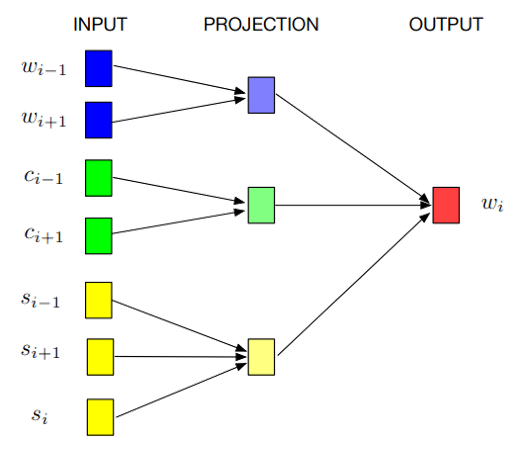
\includegraphics[scale=0.7]{../images/jwe_illustration.png}
	\caption{An illustration of JWE model proposed in \cite{yu2017joint}}
	\label{fig:jwe}
\end{figure}

As shown in the Figure \ref{fig:jwe} above, The JWE model is trained to predicts the present word from the context words in the same way as CBOW. The symbol $w$ represents words, $w_i$ is the current word, $w_{i-1}$ and $w_{i+1}$ are the context words. The symbol $c$ represents the characters of context words, $c_{i-1}$ is the characters of $w{i-1}$, and $c_{i+1}$ is the characters of $c_{i+1}$. The symbol $s$ represents the sub-characters of context words. $s_i$ is the sub-character components of $w_i$, and $s_{i-1}, s_{i+1}$ are the components of $w_{i-1}$ and $w_{i+1}$. For example, a word 智能 (intelligence) has two characters 智 (wisdom) and 能 (able), and each has sub-character components: 知, 日 and ㄙ, 月, 匕, 匕. The JWE model aims to maximize the sum of log-likelihoods of 3 conditional probabilities that come from the context words ($h_{i1}$), characters ($h_{i2}$), and sub-characters ($h_{i3}$).

\begin{equation}
L(w_i) = \sum_{k=1}^3\log P(w_i\mid h_{ik})    
\end{equation}

\subsubsection{cw2vec Model}

Inspired by fastText \cite{bojanowski2017enriching}, the authors of cw2vec \cite{cao2018cw2vec} proposed an n-gram feature based on the strokes of Chinese characters. They first split and transformed the text into stroke information, and mapped the strokes into 5 corresponding stroke ids, then merge the ids and generate n-gram features from these stroke ids. The diagram in the paper (Figure \ref{fig:cw2vec1}) shows the complete process.

\begin{figure}[h]
	\centering
	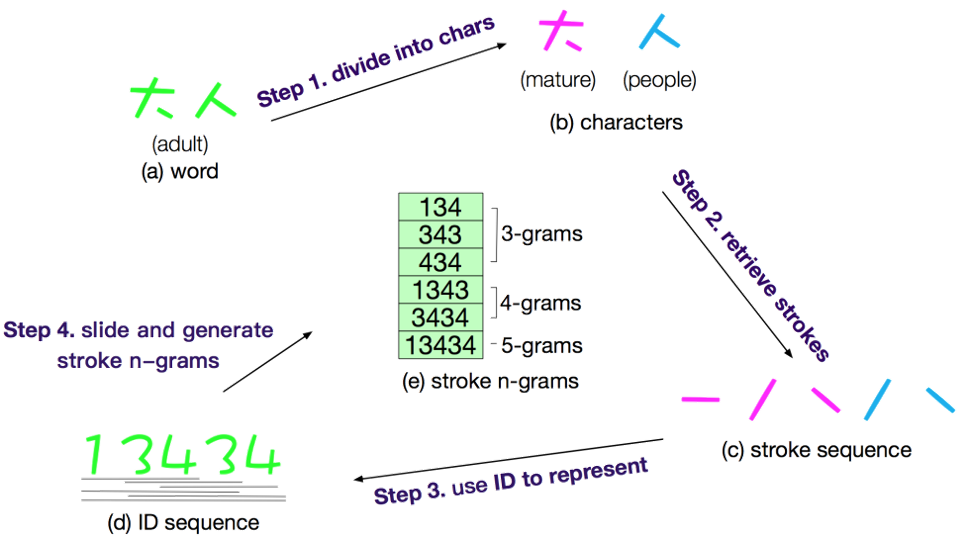
\includegraphics[scale=0.6]{../images/cw2vec_illustration1.png}
	\caption{The Process of generating stroke n-grams shown in \cite{cao2018cw2vec}}
	\label{fig:cw2vec1}
\end{figure}

The authors used Skip-Gram, a second method other than CBOW proposed by Word2Vec \cite{mikolov2013efficient}, as the base model, and replaced word inputs with stroke n-grams (Figure \ref{fig:cw2vec2}). It is mentioned in the paper that the final embeddings come from the contextual word vectors.

\begin{figure}[h]
	\centering
	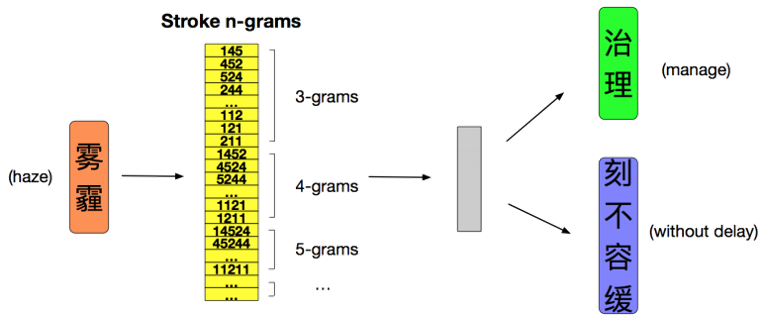
\includegraphics[scale=0.6]{../images/cw2vec_illustration2.png}
	\caption{An illustration of cw2vec model proposed in \cite{cao2018cw2vec}}
	\label{fig:cw2vec2}
\end{figure}

These word embeddings designed for Chinese all utilized the radicals or strokes in Chinese characters. No research in Chinese word embeddings has so far used phonetic information extracted from Chinese or Japanese as features.

\subsection{Phonetic Word Embedding} \label{sec:rw_pwe}

We will review studies that use phonetic information to construct word embeddings. These studies are closely related to our research, and we will learn from their practical differences and use them as the cornerstone for our experiments.

\subsubsection{Phonetic Encoding}

The study \cite{khan2019diversity} extracted sentences from Chinese or Western languages into phonetic encodings \footnote{The logogram encoding is also used as a feature but is not explained here. Random clustering is used for comparison purposes.}, which used \textit{Soundex}, \textit{NYSIIS}, \textit{Metaphone}, and \textit{Hanyu Pinyin} as the extraction algorithm. After that, they applied BPE \cite{sennrich_neural_2016} to tokenize the sentences and encodings, and trained separate embeddings from the sentences and each encoding (empty boxes in Figure \ref{fig:phonetic1}). Lastly, they concatenated the embeddings and fed them into the NMT system. 

\begin{figure}[h]
	\centering
	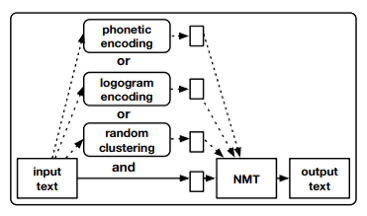
\includegraphics[scale=0.9]{../images/phonetic_encoding.png}
	\caption{Implementation of phonetic encoding proposed in \cite{khan2019diversity}}
	\label{fig:phonetic1}
\end{figure}

This paper did not explain the implementation of phonetic information in detail, but they had presented a hypothesis and verified it. That is, phonetics is a function that groups semantically distinct words. The words with the same pronunciation and spelling are usually distinguished by the different contexts.

\newpage

\subsubsection{Joint Textual and Phonetic Embedding}

This paper \cite{liu-etal-2019-robust} focused on using phonetic embedding to adjust the homophone noise problem, which is a frequent problem in a parallel corpus. For instance, when a single word in the source sentence is misplanted as a corresponding homophone (e.g., 有 (yǒu, to have) is wrongly replaced with 友 (yǒu, friend)), the model will read the wrong embedding and training in a wrong direction. The phonetic embedding can be seen as a feature to offset the errors that occur in semantic embeddings with homophone noise.

The paper trained the text (denoted by $a$) as semantic embedding (denoted by $\pi(a)$) and phonetic embedding (denoted by $\psi(a)$), and combined two embeddings with a configurable parameter (denoted by $\beta$) as follows:

\begin{equation}
	\pi([a, \psi(a)]) = (1-\beta) \times \pi(a) + \beta \times \pi(\psi(a)) 
\end{equation}

This study did not give the details of constructing embeddings, but they had mentioned that the best result occurs when the $\beta$ is $0.95$. That is, when they used 5\% of semantic embedding and 95\% of phonetic embedding, they obtained the best performance in their NMT system.

To summarize the findings in these related works. The phonetic encodings can emphasize the difference between semantically diverse sentences. The joint semantic-phonetic embedding also shows the robustness to noise in parallel corpora. All of these features can help improve the performance of the NMT system. However, the methods of using phonetic information as embeddings had been explored mainly in Chinese and Western languages. They also used \textit{Pinyin} instead of Bopomofo as the component to decompose Chinese characters. According to our study, no research has been proposed to apply and analyze phonetic information as an additional feature in Chinese and Japanese NMT systems.


\chapter{Method} \label{ch:method}
	\hspace{24pt}

This paper attempts to improve the zh-ja NMT system by utilizing the phonetic information hidden in the sentences. Section~\ref{sec:tokenization} explains which tokenization methods we use to deconstruct sentences. Section~\ref{sec:phonetic_data} explains which phonetic extraction methods we use to transform plain sentences into phonetic encodings. Section~\ref{sec:embedding} shows how we use Word2Vec as our algorithm to build and combine semantic and phonetic embeddings. Section~\ref{sec:corpus_filtering} shows how we process data from the corpus to eliminate as much noise and reduce the size of the corpus as possible. Section~\ref{sec:nmt_model} explains the details of two NMT models, which are the Attention-based GRU encoder-decoder Model and Transformer. Section~\ref{sec:embedding_analysis} describes the methods we use to analyze the difference between semantic embeddings and joint semantic-phonetic embeddings.

\section{Tokenization} \label{sec:tokenization}

This paper will examine the effectiveness of phonetic information under different tokenization methods. We use the \textit{tokenizers} \footnote{https://github.com/huggingface/tokenizers} library from the \textit{huggingface} team as our main framework for tokenization. SentencePiece \footnote{https://github.com/google/sentencepiece}, Jieba, and Janome can be implemented as pre-tokenizers in Huggingface Tokenizers.

\subsection{Huggingface Tokenizers} \label{sec:tokenizers}

Huggingface Tokenizers has 5 components that allow users to customize their tokenization methods. These five components are normalizers, pre-tokenizers, models, post-processors, and decoders. Normalizers process an input string such as lower cases or remove spaces and symbols to make it normalized. Pre-tokenizers split an input string according to a set of rules, and pre-tokenizers are where we apply SentencePiece, Jieba, and Janome. Models are responsible for converting text into ids by using the rules learned in the corpus (e.g., WordPiece, BPE, Unigram). Post-processors help us to insert special tokens into the sentence, such as the start token \textit{[BOS]} and the end token \text{[EOS]} in NMT tasks. Lastly, the job of Decoders is to reverse the ids to the original sentence.

\subsection{Byte-Pair Encoding (BPE)} \label{sec:bpe}

We use BPE as the model for merging Chinese and Japanese tokens. BPE builds a dictionary of all the words in the corpus and merges the most frequent words to generate new tokens until the maximum number of our dictionary is reached. We demonstrate the basic flow of BPE applied to Chinese through Table \ref{tab:bpe1} and \ref{tab:bpe2}.  

\vspace{0.5cm}
\begin{CJK}{UTF8}{gbsn}
\begin{table}[h]
    \centering
    \begin{tabularx}{.9\textwidth}{sbb}\toprule
        Frequency & Vocabulary & Dictionary \\
        5 & 区\enspace\_ & \_,\enspace区,\enspace地,\enspace经,\enspace济 \\
        7 & 地\enspace区\enspace\_& \\
        3 & 地\enspace区\enspace经\enspace济\enspace\_ & \\
        6 & 经\enspace济\enspace\_ & \\
        \bottomrule
    \end{tabularx}
    \caption{A simple dataset for demonstrating BPE tokenization}
    \label{tab:bpe1}
\end{table}
\end{CJK}

Words are first tokenized by pre-tokenizers and loaded into the BPE vocabulary, with the underscore (\_) representing the end of the words.

\vspace{0.5cm}
\begin{CJK}{UTF8}{gbsn}
    \begin{table}[h]
        \centering
        \begin{tabularx}{.9\textwidth}{ssb}\toprule
            Total Frequency & Merge & New Dictionary \\
            12 & (区,\enspace\_) & \_,\enspace区,\enspace地,\enspace经,\enspace济,\enspace区\_ \\
            9  & (济,\enspace\_) & \_,\enspace区,\enspace地,\enspace经,\enspace济,\enspace区\_,\enspace济\_ \\
            9  & (经,\enspace济\_) & \_,\enspace区,\enspace地,\enspace经,\enspace济,\enspace区\_,\enspace济\_,\enspace经济\_ \\
            7  & (地,\enspace区\_) & \_,\enspace区,\enspace地,\enspace经,\enspace济,\enspace区\_,\enspace济\_,\enspace经济\_,\enspace地区\_ \\
            \bottomrule
        \end{tabularx}
        \caption{The process of merging tokens in BPE tokenization}
        \label{tab:bpe2}
    \end{table}
\end{CJK}

\begin{CJK}{UTF8}{gbsn}
The merge begins with 区 and \_, which appear most frequently in the vocabulary. After merging, 区\_ will be added to the final dictionary and replaces (区\enspace\_) in the vocabulary. This process continues until the final dictionary reaches its maximum size.
\end{CJK}

\subsection{SentencePiece} \label{sec:sentencepiece}

SentencePiece treats all text in the same Unicode format. It will escape the white space with a meta symbol `\_' (U+2581). Therefore, the sentences in Chinese, Japanese, and English are considered to be in the same format, which achieving language independence. 

SentencePiece is a purely data-driven method, which means it relies on the corpus to learn the tokenization. It is simple to implement SentencePiece in Huggingface Tokenizers. First, Normalization Form Compatibility Composition (NFKC) normalizes the sentence, for example, by converting a symbol or text in the full-width form to a normalized form. Second, Metaspace pre-tokenizer splits the sentence by white space and converts the white space into the `\_' symbol. Last, BPE with dropout is applied to train with the corpus file. The dropout method will improve the robustness and accuracy.

\vspace{0.5cm}

\begin{python}
from tokenizers.normalizers import NFKC
from tokenizers import Tokenizer, pre_tokenizers, decoders, trainers

tokenizer = Tokenizer(BPE(dropout=dropout, unk_token="[UNK]"))
tokenizer.normalizer = NFKC()
tokenizer.pre_tokenizer = pre_tokenizers.Metaspace(replacement="_", add_prefix_space=True)
tokenizer.decoder = decoders.Metaspace(replacement="_", add_prefix_space=True)

trainer = trainers.BpeTrainer(vocab_size=vocab_size)
tokenizer.train(corpus, trainer=trainer)
\end{python}

\subsection{Jieba} \label{sec:jieba}

Jieba is a famous Chinese tokenization Python library that has more than 26,000 stars on Github currently. Jieba uses a prefix dictionary to store the words and calculates the longest path from the Directed Acyclic Graph (DAG) created by the sentences and dictionary to return the most likely tokenized words. In addition, Jieba uses Hidden Markov Model (HMM) and Viterbi algorithm to tokenized the unknown words in the prefix dictionary. There are four states (B, M, E, S) in the HMM model, which represent the beginning, middle, end, and single (the character can represent a word) of a character. The Viterbi algorithm takes all the words as observation and outputs the states of each character from the input sentence. 

A single line of code \pythoninline{jieba.tokenize(sentence_str)} can obtain the tokenized words from Jieba. We inserted it into Huggingface Tokenizers as a pre-tokenizer and trained the Chinese dictionary using BPE.

\vspace{0.5cm}

\begin{python}
    class JiebaPreTokenizer:
    def jieba_split(self, i: int, normalized_string: NormalizedString) -> List[NormalizedString]:
        splits = []
        for _, start, stop in jieba.tokenize(str(normalized_string)):
            splits.append(normalized_string[start:stop])
        return splits
    
    def pre_tokenize(self, pretok: PreTokenizedString):
         pretok.split(self.jieba_split)
\end{python}

\newpage

\subsection{Janome} \label{sec:janome}

Janome is a Japanese tokenization Python library that currently has 600 stars on Github. It applied the Japanese dictionary of another famous tokenization library, mecab \footnote{https://github.com/taku910/mecab}. For the methodology, Janome used the Minimal Acyclic Subsequential Transducer (MAST) as the internal dictionary data structure and the Viterbi algorithm to calculate the probability of tokenized words.

We inserted the Janome tokenizer as a pre-tokenizer to Huggingface Tokenizers and trained the Japanese dictionary using BPE.

\vspace{0.3cm}

\begin{python}
ja_tokenizer = janome.tokenizer.Tokenizer()

class JanomePreTokenizer:
    def janome_split(self, i: int, normalized_string: NormalizedString) -> List[NormalizedString]:
        splits = []
        i = 0
        for token in ja_tokenizer.tokenize(str(normalized_string).strip(), wakati=True):
            splits.append(normalized_string[i: i+len(token)])
            i += len(token)
        return splits
    
    def pre_tokenize(self, pretok: PreTokenizedString):
        pretok.split(self.janome_split)

\end{python}

\subsection{Comparison of Tokenizers} \label{sec:compare_tokenizers}

A sample of tokenized sentences using three tokenizers is listed in Table~\ref{tab:tokenized_sentences}. Jieba and Janome can tokenize the words more precisely than SentencePiece. The better performance of Jieba and Janome over SentencePiece can be considered to be due to the small size and domain specificity of the corpus.

\vspace{0.4cm}
\begin{CJK}{UTF8}{gbsn}
    \begin{table}[h]
        \centering
        \begin{tabularx}{\textwidth}{lb}\toprule
            Input (Chinese) & 平成15年进行的研究内容如下。\\
            SentencePiece & [\_平成, \_15, \_年, 进行的研究, 内容, 如下, \_。] \\
            Jieba & [平成, 15, 年, 进行, 的, 研究, 内容, 如下, 。] \\\midrule
            Input (Japanese) & 平成15年度に行なった研究内容は次の通りである。 \\
            SentencePiece & [\_平成, \_15, \_年度, に行, なった, 研究, 内容, は次の通りである, \_。] \\
            Janome & [平成, 15, 年度, に, 行なっ, た, 研究, 内容, は, 次, の, 通り, で, ある, 。] \\
            \bottomrule
        \end{tabularx}
        \caption{Tokenized sentences using three tokenizers}
        \label{tab:tokenized_sentences}
    \end{table}
\end{CJK}

\newpage

\section{Phonetic Data Extraction} \label{sec:phonetic_data}

Dragonmapper \footnote{https://github.com/tsroten/dragonmapper} is used to extract information from Chinese sentences. Pykakasi \footnote{https://github.com/miurahr/pykakasi} is used to extract information from Japanese sentences.

\subsection{Dragonmapper} \label{sec:dragonmapper}

Dragonmapper is a Python library that can convert between Chinese characters, Bopomofo, Pinyin, and International Phonetic Alphabet (IPA). When we call \pythoninline{dragonmapper.hanzi.to_pinyin(chinese_str)}, it will convert the Chinese sentence to Bopomofo tokens based on \textit{CC-CEDICT} \footnote{https://cc-cedict.org/wiki/} and \textit{Unihan} \footnote{http://www.unicode.org/charts/unihan.html} database. Table \ref{tab:dragonmapper} shows the result of phonetic extraction in Chinese sentences. The extraction will be applied to the tokenized sentences to achieve better accuracy.

\vspace{0.2cm}

    \begin{table}[h]
        \centering

        \begin{CJK*}{UTF8}{gbsn}
            \begin{tabular}{p{2.3cm}p{12cm}}\toprule
                Input & 数据详细计量对于节能推进的重要性 \\
                Tokenized & [数据, 详细, 计量, 对于, 节能, 推进, 的, 重要性] \\
            \end{tabular}
        \end{CJK*}
        
        \begin{CJK}{UTF8}{bsmi}
        \begin{tabular}{p{2.3cm}p{12cm}}
            Extracted & [ㄕㄨˋ ㄐㄩˋ,\enspace
            ㄒㄧㄤˊ ㄒㄧˋ,\enspaceㄐㄧˋ ㄌㄧㄤˋ,\enspaceㄉㄨㄟˋ ㄩˊ,\enspaceㄐㄧㄝˊ ㄋㄥˊ,\enspaceㄊㄨㄟ ㄐㄧㄣˋ,\enspaceㄉㄜ˙,\enspaceㄓㄨㄥˋ ㄧㄠˋ ㄒㄧㄥˋ]
        \end{tabular}
        \end{CJK}

        \begin{CJK*}{UTF8}{gbsn}
            \begin{tabular}{p{2.3cm}p{12cm}}\toprule
                Input & 分析项目是1997-2001年是砷、镍、锰、铬、铍 \\
                Tokenized & [分析, 项目, 在, 1997, -, 2001, 年, 是, 砷, 、, 镍, 、, 锰, 、, 铬, 、, 铍] \\
            \end{tabular}
        \end{CJK*}
        
        \begin{CJK}{UTF8}{bsmi}
        \begin{tabular}{p{2.3cm}p{12cm}}
            Extracted & [ㄈㄣ ㄒㄧ,\enspaceㄒㄧㄤˋ ㄇㄨˋ,\enspaceㄗㄞˋ,\enspace1997,\enspace-,\enspace2001,\enspaceㄋㄧㄢˊ,\enspaceㄕˋ,\enspaceㄕㄣ,\enspace、,\enspaceㄋㄧㄝˋ,\enspace、,\enspaceㄇㄥˇ,\enspace、,\enspaceㄍㄜˋ,\enspace、,\enspaceㄆㄧ]
        \end{tabular}
        \end{CJK}

        \begin{CJK*}{UTF8}{gbsn}
            \begin{tabular}{p{2.3cm}p{12cm}}\toprule
                Heteronym Test & 长大很快乐,音乐很长久 \\
                Tokenized & [长大, 很, 快乐, ,, 音乐, 很, 长久] \\
            \end{tabular}
        \end{CJK*}
        
        \begin{CJK}{UTF8}{bsmi}
        \begin{tabular}{p{2.3cm}p{12cm}}
            Extracted & ['ㄓㄤˇ ㄉㄚˋ,\enspaceㄏㄣˇ,\enspaceㄎㄨㄞˋ ㄌㄜˋ,\enspace,,\enspaceㄧㄣ ㄩㄝˋ,\enspaceㄏㄣˇ,\enspaceㄔㄤˊ ㄐㄧㄡˇ] \\\bottomrule
        \end{tabular}
        \end{CJK}

        \caption{Chinese Phonetic Extraction using Dragonmapper library}
        \label{tab:dragonmapper}
    \end{table}

\subsection{Pykakasi} \label{sec:pykakasi}

Pykakasi is a Python library that implements algorithms in \textit{kakasi} \footnote{http://kakasi.namazu.org/index.html.en} library. It is able to convert Kanji characters to Hiragana, Katakana, and Romaji through the SKK Japanese dictionary \footnote{https://github.com/skk-dev/dict} and UniDic \footnote{https://unidic.ninjal.ac.jp/}. Table \ref{tab:pykakasi} shows the result of phonetic extraction in Japanese tokenized sentences. 

\vspace{0.2cm}

\begin{CJK}{UTF8}{long}
    \begin{table}[h]
        \centering
            \begin{tabular}{p{2.3cm}p{12cm}}\toprule
                Input & 技術以外にも,政策、法律、社会的側面の課題がある \\
                Tokenized & [技術, 以外, に, も, ,, 政策, 、, 法律, 、, 社会, 的, 側面, の, 課題, が, ある] \\
                Extracted & [ぎじゅつ,\enspaceいがい,\enspaceに,\enspaceも,\enspace,,\enspaceせいさく,\enspace、,\enspaceほうりつ,\enspace、,\enspaceしゃかい,\enspaceてき,\enspaceそくめん,\enspaceの,\enspaceかだい,\enspaceが,\enspaceある] \\\midrule

                Input & 冠状動脈レントゲンでTIMI血流3級が示された \\
                Tokenized & [冠状, 動脈, レントゲン, で, TI, MI, 血流, 3, 級, が, 示さ, れ, た] \\
                Extracted & [かんじょう,\enspaceどうみゃく,\enspaceれんとげん,\enspaceで,\enspace TI,\enspace MI,\enspaceけつりゅう,\enspace3,\enspaceきゅう,\enspaceが,\enspaceしめさ,\enspaceれ,\enspaceた]\\\midrule

                Heteronym Test & 一生,芝生で生ビールを飲む \\
                Tokenized & [一生, ,, 芝生, で, 生, ビール, を, 飲む] \\
                Extracted & [いっしょう, ,, しばふ, で, なま, びーる, を, のむ] \\\bottomrule

            \end{tabular}
        \caption{Japanese Phonetic Extraction using Pykakasi library}
        \label{tab:pykakasi}
    \end{table}
\end{CJK}

% https://bamtercelboo.github.io/2018/03/24/word2vec/
\section{Embedding} \label{sec:embedding}

This paper uses Word2Vec as an embedding framework. Embedding is a distribution representation of words. Compared to using sparse vectors such as one-hot representations to represent words, embedding can represent words as high-dimensional vectors of real numbers. These vectors can be used to obtain similarity between words by computing distances such as cosine similarity. 

First, We will explore the details of Word2Vec. Second, we explain how to train a general word embedding with semantics from a corpus. Third, we examine how to manipulate the phonetic information to build a phonetic embedding. Finally, we combine two embeddings to a joint embedding which can have both semantic and phonetic information.

\subsection{Word2Vec} \label{sec:word2vec}

Word2Vec has two classic papers. The first one \cite{mikolov2013efficient} contributes two approaches to constructing an embedding, namely CBOW and Skip-gram. The second one \cite{mikolov2013distributed} contributes the improved methods of embedding construction, such as Hierarchical Softmax and Negative Sampling. We will use Skip-gram and Negative Sampling to generate word embeddings in this paper.

Skip-gram model uses a neural network with hidden layers to predict the likelihood of context words $w_{t-2}, w_{t-1}, w_{t+1}, w_{t+2}$ of an input word $w_t$. The input word and context words will be paired, such as $(w_t, w_{t-2}), (w_t, w_{t-1})$ to perform supervised training. The model can be expressed as the following equation, where $\theta$ represents hidden states of the input word $w_\text{center}$, and $w_1, w_2, \cdots, w_C$ represents the context words of $w_\text{center}$ within the window size $C$. 

% The goal is to maximize the likelihood of the occurrence of context words for each word $w$ in the corpus by updating $\theta$ iteratively.

\begin{equation}
\underset{\theta}{\operatorname{argmax}} \, p\left(w_{1}, w_{2}, \ldots, w_{C} \mid w_{\text {center}} ; \theta\right)
\end{equation}

Skip-gram uses the softmax model for context word classification. $h$ is the hidden layer word vector for the input word $w_\text{center}$ from the input embedding matrix, and $W_{\text {output}}$ is a row vector for a context word from the output embedding matrix. $W_{\text {output}_{(c)}}$ corresponds to the row vector of the context word in (input, context) pair, while $W_{\text {output}_{(i)}}$ corresponds to the row vector of each word in the corpus of size $V$.

\begin{equation}
    p\left(w_{\text {context}} \mid w_{\text {center}}\right)=\frac{\exp \left(W_{\text {output}_{{(c)}}} \cdot h\right)}{\sum_{i=1}^{V} \exp \left(W_{\text {output}_{(i)}} \cdot h\right)} \in \mathbb{R}^{1}
\end{equation}

The goal is to obtain the conditional probability distribution of each unique word observed in the corpus given an input word.

\begin{equation}
    \left[\begin{array}{c}
    p\left(w_{1} \mid w_{\text {input}}\right) \\
    p\left(w_{2} \mid w_{\text {input}}\right) \\
    p\left(w_{3} \mid w_{\text {input}}\right) \\
    \vdots \\
    p\left(w_{V} \mid w_{\text {input}}\right)
    \end{array}\right]=\frac{\exp \left(W_{\text {output }_{(c)}} \cdot h\right)}{\sum_{i=1}^{V} \exp \left(W_{\text {output }_{(i)}} \cdot h\right)} \in \mathbb{R}^{V}
\end{equation}

In machine learning, it is a convention to minimize the loss function. The log is added to the equation to simplify and accelerate the calculation, and the formula is rewritten as minimizing a negative log-likelihood instead of maximizing a positive log-likelihood.

\begin{align}
J\left(\theta ; w^{(t)}\right)&=-\log \prod_{c=1}^{C} \frac{\exp \left(W_{\text {output }_{(c)}} \cdot h\right)}{\sum_{i=1}^{V} \exp \left(W_{\text {output }_{(i)}} \cdot h\right)} \\
&=-\sum_{c=1}^{C} \log \frac{\exp \left(W_{\text {output }_{(c)}} \cdot h\right)}{\sum_{i=1}^{V} \exp \left(W_{\text {output }_{(i)}} \cdot h\right)} \\
&=-\sum_{c=1}^{C}\left(W_{\text {output }_{(c)}} \cdot h\right)+C \cdot \log \sum_{i=1}^{V} \exp \left(W_{\text {output }_{(i)}} \cdot h\right)
\end{align}

Figure~\ref{fig:skip-gram} shows the Skip-gram model. we will learn word embedding vectors of size $N$ given the vocabulary size $V$. The model uses one input word at a time for learning to predict one context word (output).

\begin{figure}[h]
	\centering
	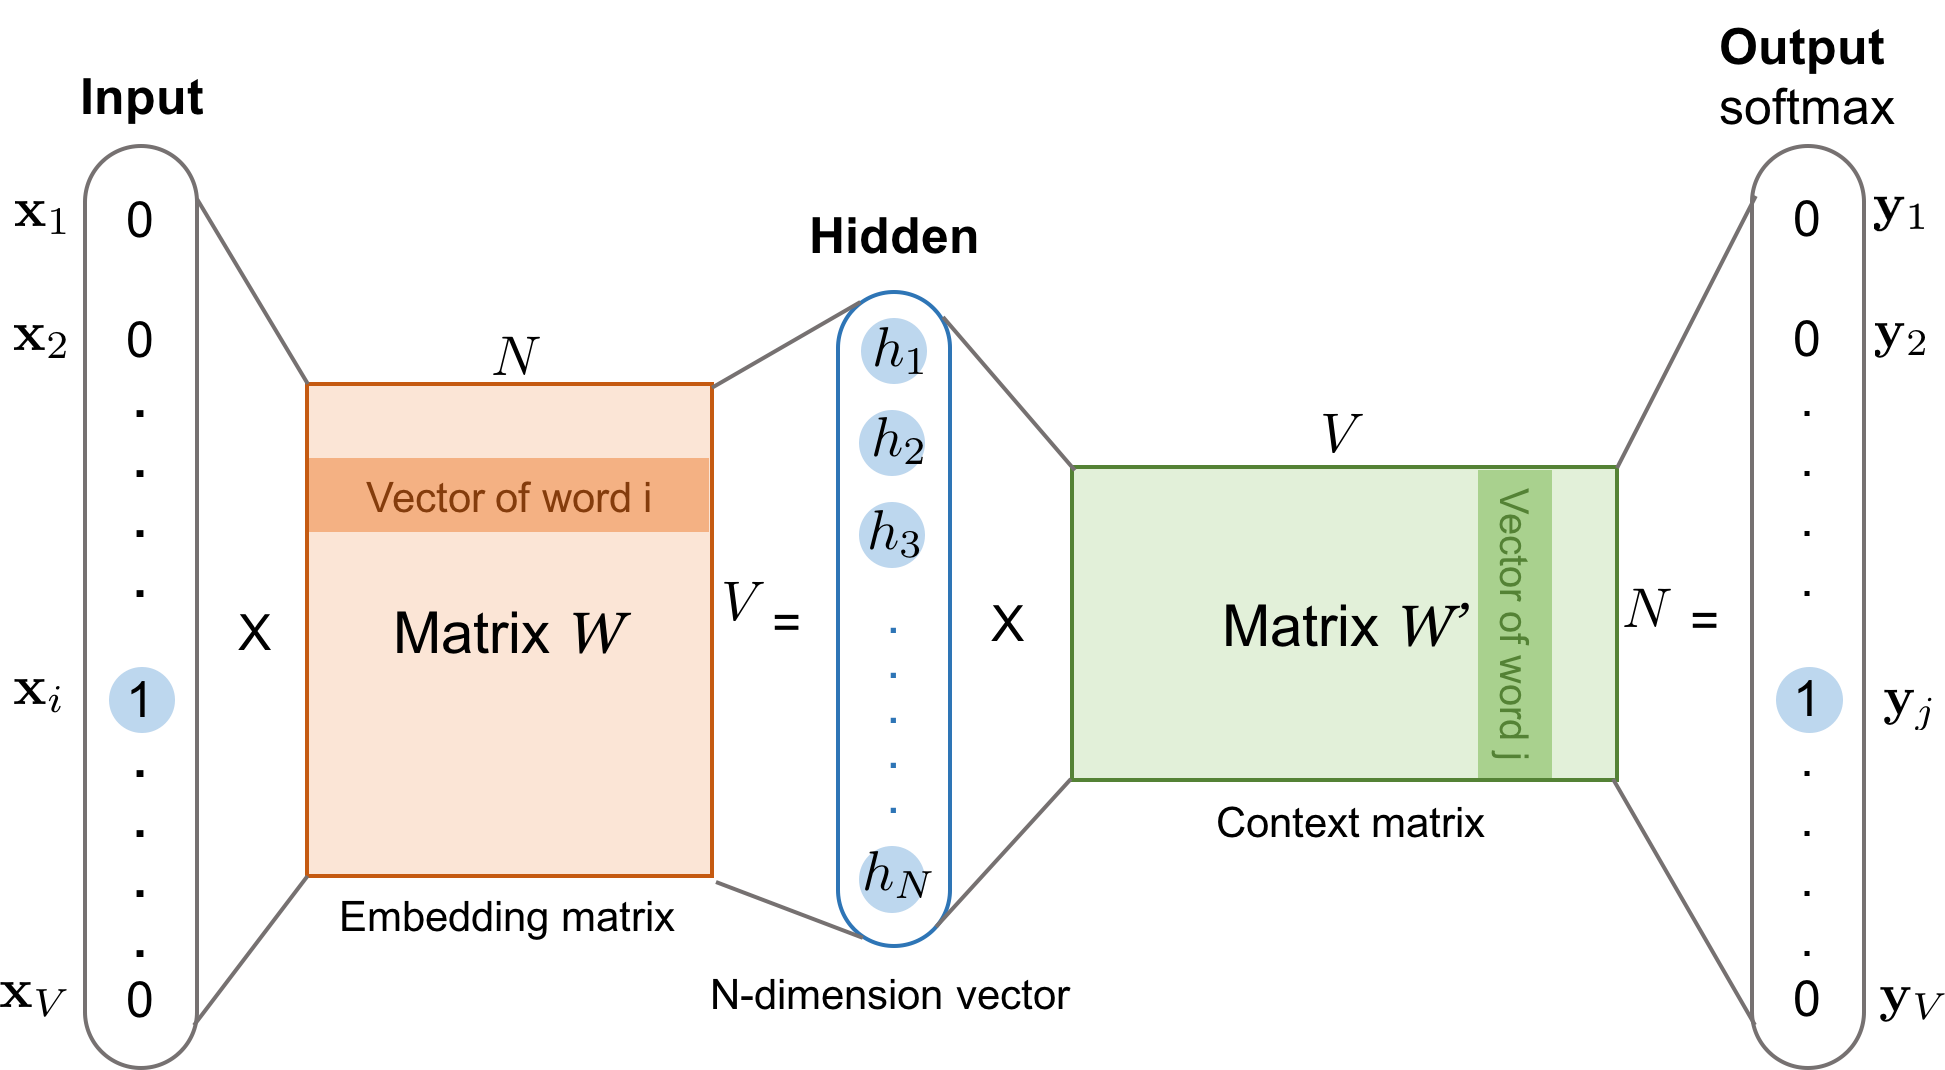
\includegraphics[scale=0.4]{../images/skip-gram.png}
    \caption[The Skip-gram Model]{The Skip-gram Model\protect\footnotemark}
	\label{fig:skip-gram}
\end{figure}

\footnotetext{Source: https://lilianweng.github.io/lil-log/2017/10/15/learning-word-embedding.html}

Since the softmax model requires a lot of computational space and time, we also use negative sampling with the Skip-gram model. Negative sampling will convert the multi-classification problem that the model is designed to solve into a binary-classification problem. First, the method will randomly select $K$ negative samples from the corpus that are irrelevant to the input word. $K$ is a hyper-parameter, usually between 5 and 20. The model will update $(K+1)\times N$ parameters using the sigmoid function, where $N$ is the dimension of the hidden layer $h$, and $+1$ accounts for the positive sample.

The probability that a word ($c$) appears within the context of the input word ($w$) can be defined as the following formula. The goal is to determine whether $c$ is in the context window of $w$ ($D=1$) or not ($D=0$) based on the input-context pairs $(w, c)$.

\begin{equation}
p(D=1 \mid w, c ; \theta)=\frac{1}{1+\exp \left(-\bar{c}_{\text {output }_{(j)}} \cdot w\right)} \in \mathbb{R}^{1}
\end{equation}

\subsection{Semantic Embedding}

We use gensim to implement Skip-gram with negative sampling from Word2Vec. We put the tokenized sentences generated by different tokenizers into gensim to train the general word embedding with semantics. The following are the main settings of the parameters: \textit{max\_vocab\_size} is 32000, \textit{vector\_size} is 300, \textit{epoch\_number} is 13, \textit{window\_size} is 5, the number of negative samples is 5, ignoring the words with total frequency lower than 5.

Some words may not be trained in the model, such as special tokens and low-frequency words. Therefore, the size of the trained embedding matrix and the tokenizer vocabulary is not identical, resulting in different coverage (Table~\ref{tab:semantic_coverage}). We calculate the mean and standard deviation of the whole embedding and randomly assign the empty word vectors using the normal distribution.

\vspace{0.5cm}
\begin{table}[h]
    \centering
    \begin{tabularx}{.9\textwidth}{ssss}\toprule
        Language & SentencePiece & Jieba & Janome \\\midrule
        Chinese & 95\% (30368/32000) & 93\% (29613/32000) & - \\
        Japanese & 97\% (30940/32000) & - & 93\% (29801/32000) \\
        \bottomrule
    \end{tabularx}
    \caption{The coverage of semantic embedding in vocabulary}
    \label{tab:semantic_coverage}
\end{table}

\subsection{Phonetic Embedding} \label{sec:phonetic_embedding}

The training method for phonetic embedding is mostly the same as semantic embedding. First, we convert tokenized sentences into phonetic encodings using the phonetic extraction techniques described in Section~\ref{sec:phonetic_data}. Second, we adopt the same training methods and parameters from semantic embedding. And last, we share the same vector of characters or words with the same pronunciation or spelling in the embedding matrix. Therefore, the coverage (Table~\ref{tab:phonetic_coverage}) will be even higher than the semantic embedding. The empty vectors are also randomly assigned using the normal distribution with mean and standard deviation from the whole embedding. 

\vspace{0.5cm}
\begin{table}[h]
    \centering
    \begin{tabularx}{.9\textwidth}{ssss}\toprule
        Language & SentencePiece & Jieba & Janome \\\midrule
        Chinese & 99\% (31753/32000) & 97\% (31068/32000) & - \\
        Japanese & 99\% (31698/32000) & - & 96\% (30809/32000) \\
        \bottomrule
    \end{tabularx}
    \caption{The coverage of phonetic embedding in vocabulary}
    \label{tab:phonetic_coverage}
\end{table}

\subsection{Joint Embedding} \label{sec:joint_embedding}

Several ways have been proposed to combine multiple embeddings, such as concatenation, training and blending separate embedding using the same model, and meta-embedding. Meta-embedding is a very vague term, but the core idea is to accept any kind of pre-trained embedding and fuse them into one (meta) embedding. Many studies on meta-embedding have been proposed \cite{kiela-etal-2018-dynamic, yin2015learning, muromagi2017linear}. The methods of meta-embedding can range from very complicated to very straightforward. This paper uses a simple averaging method \cite{coates-bollegala-2018-frustratingly} to merge semantic and phonetic embedding.

\section{Corpus Filtering} \label{sec:corpus_filtering}

We define custom rules and apply alignment scores from \textit{fast\_align} \cite{dyer2013simple} to perform corpus filtering to reduce noise, dataset size, and resource burden during training in the NMT system. The original dataset had 672,315 sentence pairs, which were reduced to 557,685 using rules and 462,582 using alignment scores.

\subsection{Pre-filtering rules}

We apply the following rules to exclude the pairs of sentences that do not match:

\begin{enumerate}
    \item Removing sentences that are too large in proportion to their length.
    \item Removing sentences that are too short or too long.
    \item Removing identical sentences.
    \item Removing sentences that cannot be correctly identified as Chinese or Japanese by the fastText identification model.
    \item Removing sentences with more English and numeric characters than Chinese and Japanese.
    \item Removing sentences that have more than one counterpart.
\end{enumerate}

\subsection{Scoring functions}

fast\_align is a tool based on \textit{IBM alignment model 2} for training statistical machine translation and alignment model. The score is the probability of the source sentence given the target sentence and its alignment. The algorithm iteratively estimates the probability of being each other translation for source-target pairs and optimal alignment given the word-to-word translation probabilities. 

In theory, the score should correlate with the degree of parallelism of the sentences. We remove the sentence pairs that are below a certain probability score threshold as shown in Table~\ref{tab:alignment_scores}. 

\newpage

\begin{table}[h]
    \centering
    \begin{tabularx}{.7\textwidth}{ss}\toprule
        Alignment Score Range & Number of sentence pairs \\\midrule
        $[-3, -81]$ & 173,100 \\
        $[-81, -160]$ & 287,882 \\\midrule
        $[-160, -238]$ & 93,134 \\
        $[-238, -317]$ & 3,540 \\
        $[-317, -395]$ & 29 \\
        \bottomrule
    \end{tabularx}
    \caption{Distribution of Sentence Pair Alignment Scores}
    \label{tab:alignment_scores}
\end{table}

We sampled some sentence pairs corresponding to alignment scores in Table~\ref{tab:alignment_samples}. The findings were that the lower the score, the longer the sentences tended to be, the more words were not translated, and the higher the proportion of proper nouns became.

\vspace{0.3cm}
\begin{table}[h]
    \centering
    \begin{CJK}{UTF8}{gbsn}
        \begin{tabularx}{\textwidth}{lb}\toprule
            Score & -52 \\
            {Chinese } & 残留性化学物质的物质循环模型的构建和再利用·废弃物政策评价的应用 \\
        \end{tabularx}
    \end{CJK}
    \begin{CJK}{UTF8}{long}
        \begin{tabularx}{\textwidth}{lb}
            Japanese & 残留性化学物質の物質循環モデルの構築とリサイクル・廃棄物政策評価への応用 \\
            \midrule
        \end{tabularx}
    \end{CJK}
    \begin{CJK}{UTF8}{gbsn}
        \begin{tabularx}{\textwidth}{lb}
            Score & -151 \\
            {Chinese } & 使用传统的轴组装工法的2层木制住宅,进行了室内甲醛浓度的测量,同时也研讨了上下楼层的甲醛浓度和换气量的关系。 \\
        \end{tabularx}
    \end{CJK}
    \begin{CJK}{UTF8}{long}
        \begin{tabularx}{\textwidth}{lb}
            Japanese & 在来軸組工法木造2階建住宅を用いて,室内ホルムアルデヒド濃度の測定を行うとともに,上下階のホルムアルデヒド濃度と換気量の関係も検討した。 \\
            \midrule
        \end{tabularx}
    \end{CJK}
    \begin{CJK}{UTF8}{gbsn}
        \begin{tabularx}{\textwidth}{lb}
            Score & -254 \\
            {Chinese } & 当我尽快编写了PID控制程序并运行后发现,不仅温度不能很好地稳定,还出现了“不规则振荡”现象(重复出现大幅度偏离控制值的振动),控制彻底失败了。 \\
        \end{tabularx}
    \end{CJK}
    \begin{CJK}{UTF8}{long}
        \begin{tabularx}{\textwidth}{lb}
            Japanese & 早速,PID制御のプログラムを書いて実行したところ,うまく温度が安定化しないどころかいわゆる“ハンチング”現象(制御値から大きく外れた振動を繰り返す)を起こしてしまい,見事,制御に失敗した \\
            \midrule
        \end{tabularx}
    \end{CJK}
    \begin{CJK}{UTF8}{gbsn}
        \begin{tabularx}{\textwidth}{lb}
            Score & -254 \\
            {Chinese } & ('关于葛根、黄苓、黄连汤之证,在『伤寒论』34条中叙述:“太阳病,桂枝证,医反下之,利遂不止,脉促者,表未解也,喘而汗出者,葛根黄芩黄连汤主之”。 \\
        \end{tabularx}
    \end{CJK}
    \begin{CJK}{UTF8}{long}
        \begin{tabularx}{\textwidth}{lb}
            Japanese & '葛根黄苓黄連湯証について,『傷寒論』34条に,「太陽病,桂枝の証,医反ってこれを下し,利遂に止まず,脈促のものは,表いまだ解せざるなり,ぜんして汗出づるものは,葛根黄苓黄連湯これを主る」という。 \\
            \midrule
        \end{tabularx}
    \end{CJK}
    \caption{Samples of Sentence Pairs with Alignment Scores}
    \label{tab:alignment_samples}
\end{table}


% -52 残留性化学物质的物质循环模型的构建和再利用·废弃物政策评价的应用\n',
%    '残留性化学物質の物質循環モデルの構築とリサイクル・廃棄物政策評価への応用

% -151 使用传统的轴组装工法的2层木制住宅,进行了室内甲醛浓度的测量,同时也研讨了上下楼层的甲醛浓度和换气量的关系。\n',
%    '在来軸組工法木造2階建住宅を用いて,室内ホルムアルデヒド濃度の測定を行うとともに,上下階のホルムアルデヒド濃度と換気量の関係も検討した。

% -254 当我尽快编写了PID控制程序并运行后发现,不仅温度不能很好地稳定,还出现了“不规则振荡”现象(重复出现大幅度偏离控制值的振动),控制彻底失败了。\n',
%    '早速,PID制御のプログラムを書いて実行したところ,うまく温度が安定化しないどころかいわゆる“ハンチング”現象(制御値から大きく外れた振動を繰り返す)を起こしてしまい,見事,制御に失敗した


% -338 ('关于葛根、黄苓、黄连汤之证,在『伤寒论』34条中叙述:“太阳病,桂枝证,医反下之,利遂不止,脉促者,表未解也,喘而汗出者,葛根黄芩黄连汤主之”。\n',
% '葛根黄苓黄連湯証について,『傷寒論』34条に,「太陽病,桂枝の証,医反ってこれを下し,利遂に止まず,脈促のものは,表いまだ解せざるなり,ぜんして汗出づるものは,葛根黄苓黄連湯これを主る」という。\n')),

% 越長的句子通常會對應越低的分數

% 我們列出一些 alignment score 對應的句子對,



\section{NMT Model} \label{sec:nmt_model}

% 我們使用兩種模型來訓練 NMT 任務。分別是基於某論文提的。以及某某論文提起。模型的參數在哪裡提,模型的評分在哪裡提。模型的結果在哪裡提。關於翻譯的句子 case study 會在哪裡提。

\subsection{Attention-based GRU encoder-decoder Model} \label{sec:rnn}

% 先講所有架構。

% 分別講每個架構。每個架構的圖,公式。

\subsection{Transformer} \label{sec:transformer}

% 先講所有架構。

% 分別講每個架構。每個架構的圖,公式。

% https://bamtercelboo.github.io/2018/05/12/embedding_evaluation/
\section{Embedding Analysis} \label{sec:embedding_analysis}

% 我們使用四種方法驗證有效性。希望XX能保留效果,希望能加強 4。我們用 gensim 來實作這四個驗證。驗證結果會在 discussion 討論。

\subsection{Analogy Reasoning} \label{sec:analogy}

% 講解這個東西在幹嘛的。怎麼算。怎麼用 gensim 跑。

\subsection{Outlier Detection} \label{sec:outlier}

% 講解這個東西在幹嘛的。怎麼算。怎麼用 gensim 跑。

\subsection{Word Similarity} \label{sec:similarity}

% 講解這個東西在幹嘛的。怎麼算。怎麼用 gensim 跑。

\subsection{Homonym and Heteronym} \label{sec:homonym_heteronym}

% 講解這個東西在幹嘛的。怎麼算。怎麼用 gensim 跑。


\chapter{Experiment and Result} \label{ch:experiment_and_result}
	\hspace{24pt}

% 方法加個圖吧

% 講解整個實驗的流程。用什麼資料集。用什麼環境展開實驗。模型中用什麼參數。用什麼評分翻譯系統。所有翻譯系統的評分結果。

\section{Dataset} \label{sec:dataset}

% 講解 Dataset 的來源。內容。架構。

\section{Environment} \label{sec:environment}

% 講解執行 NMT 實驗會用到的架構和 logger。

\subsection{PyTorch Lightning} \label{sec:lightning}

% lightning 的理念,核心,好處。

\subsection{wandb} \label{sec:wandb}

% wandb 的理念,核心,好處。

\section{Parameter} \label{sec:parameter}

% 分別在兩種模型的一般參數使用哪些數值。以及 hyperparameter。還有 embedding 解凍。

\section{Metric} \label{sec:metric}

% 我們用 BLEU 做為評分標準。BLEU 是什麼,怎麼算。常見的分數解釋。

\section{Result} \label{sec:result}

% 我們以 WAT 2020 做為標準。什麼是 WAT 2020。他們同樣使用 ASPEC。分別用什麼分詞。分數為多少。

% RNN 的結果,SENTENCEPIECE 結果,LOSS,BLEU。JIEBA JANOME 結果,LOSS,BLEU。

% TRANSFORMER 的結果,SENTENCEPIECE 結果,LOSS,BLEU。JIEBA JANOME 結果,LOSS,BLEU。


\chapter{Discussion} \label{ch:discussion}
	\hspace{24pt}

% 在 case study 我們會挑選一些翻譯結果,試著解釋為什麼翻譯較好的原因。
% 在 embedding analysis 我們探討 joint 和 semantic 比對的結果。

\section{Case Study} \label{sec:case_study}

% 列個 5 種吧。講解哪些詞翻較好。哪些地方比較成功。用聲音資訊來解釋佳。

% \begin{center}
%     \begin{CJK*}{UTF8}{gbsn}
%     \begin{tabular}{p{7.3cm}p{27.5cm}} \toprule
%       Source & 微小粒子测量装置的比较试验\\\midrule
%     \end{tabular}
%     \end{CJK*}
%     \begin{CJK}{UTF8}{min}
%     \begin{tabular}{p{7.3cm}p{27.5cm}}
%       Target & 微小粒子測定装置の比較試験\\
%       Semantic & 微小粒子計測装置の比較実験 \\
%       Semantic + Phonetic & 微小粒子測定装置の比較試験\\
%     \end{tabular}
%     \end{CJK}
%     \begin{CJK*}{UTF8}{gbsn}
%     \begin{tabular}{p{7.3cm}p{27.5cm}} \toprule
%       Source & 从背景知识B和观测结果O中获得行动规则的集合Y的集合H。\\\midrule
%     \end{tabular}
%     \end{CJK*}
%     \begin{CJK}{UTF8}{min}
%     \begin{tabular}{p{7.3cm}p{27.5cm}}
%       Target & 背景知識Bと観測結果Oより行動規則の集合Yの集合を獲得する.\\
%       Semantic & 背景背景知識Bと観測結果Oから行動ルールの集合Yの集合H獲得する. \\
%       Semantic + Phonetic & 背景知識Bと観測結果Oから行動規則の集合Yの集合H獲得する.\\\bottomrule
%     \end{tabular}
%     \end{CJK}
%     \captionof{table}{\color{Green}Case Study}
%     \label{table:case_study}
%     \end{center}

\section{Embedding Analysis} \label{sec:analysis}

% 以四種方式來探討 joint embedding 的優點,與 semantic 的差異。

\subsection{Analogical Reasoning} \label{sec:analysis_analogy}

% 放上結果,講差別,不只保留字義,且超過,優點

% \begin{center}\vspace{0.3cm}
%     \begin{CJK*}{UTF8}{bsmi}
%         \begin{tabular}{P{3.5cm} P{8cm} P{8cm} P{8cm}}
%             \toprule
%             \multirow{2.5}{*}{Language} & \multirow{2.5}{*}{Input ($a:A=b:$)} & \multicolumn{2}{c}{Output ($B$)} 
%             \\\cmidrule{3-4}
%             & & Semantic Only & Semantic + Phonetic \\\midrule
%             Chinese & 東京:日本$=$北京: & 中國 \ ($p=0.49$) & 中國 \ ($p=0.53$) \\
%             {} & 長期:三年$=$短期: & 一年 \ ($p=0.38$) & 兩周 \ ($p=0.39$) \\
%             {} & 進口:買入$=$出口: & 賣出 \ ($p=0.36$) & 賣出 \ ($p=0.44$) \\\midrule
%         \end{tabular}
%     \end{CJK*}
    
%     \begin{CJK}{UTF8}{min}
%         \begin{tabular}{P{3.5cm} P{8cm} P{8cm} P{8cm}}
%             Japanese & 男性:女性$=$父親: & 母親 \ ($p=0.49$) & 母親 \ ($p=0.51$) \\
%             & 長期:年$=$短期: & 月 \ ($p=0.55$) & 月 \ ($p=0.57$) \\
%             & 左右:前後$=$水平: & 垂直 ($p=0.43$) & 垂直 ($p=0.40$) \\
%             \bottomrule
%         \end{tabular}
%     \end{CJK}
    
%     \captionof{table}{\color{Green}Analogy Test}
%     \label{table:analogy_test}
% \end{center}


\subsection{Outlier Detection} \label{sec:analysis_outlier}

% 放上結果,講差別,優點

% \begin{center}\vspace{0.3cm}
%     \begin{CJK*}{UTF8}{bsmi}
%         \begin{tabular}{P{3.5cm} P{12cm} P{6cm} P{8cm}}
%             \toprule
%             \multirow{2.5}{*}{Language} & \multirow{2.5}{*}{Input} & \multicolumn{2}{c}{Output (Outlier)} 
%             \\\cmidrule{3-4}
%             & & Semantic Only & Semantic + Phonetic \\\midrule
            
%             Chinese & 維持, 保持, 堅持, 建設  & 建設 & 建設 \\
%             {} & 可行, 不行, 可以, 行 & 可以 & 不行 \\\midrule
            
%         \end{tabular}
%     \end{CJK*}
    
%     \begin{CJK}{UTF8}{min}
%         \begin{tabular}{P{3.5cm} P{12cm} P{6cm} P{8cm}}
%         Japanese & 生み, 創造, 作る, 破壊 & 破壊 & 破壊\\
%         & 普通, 一般, 通常, 異常 & 異常 & 異常\\
%         \bottomrule
%         \end{tabular}
%     \end{CJK}
    
%     \captionof{table}{\color{Green}Outlier Detection}
%     \label{table:outlier_detection}
% \end{center}


\subsection{Word Similarity} \label{sec:analysis_similarity}

% 放上結果,講差別,優點

\subsection{Homonym and Heteronym} \label{sec:analysis_homonym_heteronym}

% 放上結果,講差別,優點



% \begin{center}\vspace{0.3cm}
%     \begin{CJK*}{UTF8}{bsmi}
%         \begin{tabular}{P{3.5cm} P{12cm} P{6cm} P{8cm}}
%             \toprule
%             \multirow{2.5}{*}{Language} & \multirow{2.5}{*}{Input} & \multicolumn{2}{c}{Distance} 
%             \\\cmidrule{3-4}
%             & & Semantic Only & Semantic + Phonetic \\\midrule
%             Chinese & 長(ㄔㄤˊ)度, 長(ㄓㄤˇ)大  & 0.826 & \textbf{0.853} \\
%             {} & 樂(ㄌㄜˋ)趣, 音樂(ㄩㄝˋ) & 0.636 & \textbf{0.682} \\
%             {} & 中(ㄓㄨㄥ)午, 中(ㄓㄨㄥˋ)毒 & 0.841 & \textbf{0.866}\\\midrule
%         \end{tabular}
%     \end{CJK*}
%     \begin{CJK}{UTF8}{min}
%         \begin{tabular}{P{3.5cm} P{12cm} P{6cm} P{8cm}}
%                 Japanese & 生(なま), 一生(しょう)  & 0.879 & \textbf{0.889} \\
%                 {} & 生(なま), 生(き)地 & 0.769 & \textbf{0.867} \\
%                 {} & 生(なま), 生(う)む & 0.829 & \textbf{0.839} \\\bottomrule
%         \end{tabular}
%     \end{CJK}
%     \captionof{table}{\color{Green}Similarity Distances Between Heteronyms}
%     \label{table:noise_heteronym}
% \end{center}

\chapter{Conclusion and Future Work} \label{ch:conclusion}
	\hspace{24pt}

This chapter will summarize the findings and contributions and further discuss some of the potential improvements to the paper. We will summarize the results and contributions in Section~\ref{sec:conclusion}. After that, we propose a series of methods that can be further studied or improved as our future work in Section~\ref{sec:future_work}.

\section{Conclusion} \label{sec:conclusion}

This paper intended to improve the neural machine translation between Chinese and Japanese by applying feature engineering to texts, constructing a word embedding with phonetic information, and combining the phonetic embedding with general word embedding that possesses semantics. The resulting joint semantic-phonetic embedding gave positive feedback in the neural machine translation model and the embedding analysis. 

In our translation task based on different models and tokenization methods, the use of joint embedding had achieved better BLEU scores than the use of semantic or phonetic embedding. Moreover, the translation results generated by the best model with joint embedding also revealed four advantages. These translations selected the correct, better text; and preserved Katakana and English text for the target sentences. As a result, these advantages have a positive connection to the joint embedding with the addition of phonetic information.

Embedding analysis further identified the effectiveness of joint embedding. The tests from analogical reasoning and outlier detection demonstrated that the joint embedding not only had retained the capabilities but also enhanced the performance of the semantic embedding. Furthermore, the similarity distance and Pearson correlation of synonyms, homonyms, and heteronyms were observed to be better in joint embedding, which indicates the improvement in semantics and noise resistance.

The success of translation task and embedding analysis revealed that the joint semantic-phonetic embedding has a certain degree of enhancement and contribution to the Chinese-Japanese neural machine translation system.

\section{Future Work} \label{sec:future_work}

% 本論文有許多能夠深入研究的方向,我們在此列出幾個方法,這些方法有的或許能進一步分析現有表現,有的或許有機會能進一步提高表現。

% 改善產生聲音資訊的方法,例如使用其他的插件來產生並比較優劣,舉例

% 採用在 related work 中提到訓練 embedding 的模式,將聲音資訊與中文字、及各種 subcharacter feature 例如筆畫、部首來一起訓練一個 embedding。

% 採用 ELMO、BERT 當作基礎的 embedding 架構。由於他們兩者都是屬於需要綁定模型的 embedding,所以可以考慮訓練一個 semantic model 和一個 phonetic model 並將兩者結合起來。

% 最新研究展示 cnn 用於 NLP 領域強於 transformer。所以我們也可以試用 CONVS2S 當作模型架構,。
\newpage
\phantomsection % for hyperref to register this
\addcontentsline{toc}{chapter}{References}
\renewcommand{\bibname}{\protect\makebox[5cm][s]{REFERENCES}}
%  \makebox{} is fragile; need protect
\bibliographystyle{apalike}
% \bibliographystyle{IEEEtranS}  % 使用 IEEE Trans 期刊格式

%% References with bibTeX database:
\bibliography{back/ncku_thesis_bib}
\baselineskip=18pt



\clearpage % to make sure all CJK characters are processed
\end{CJK}
\end{document}